\documentclass{article}
\usepackage[utf8]{inputenc}
\usepackage[margin=1in]{geometry}
\usepackage{graphicx}
\bibliographystyle{plainnat}
\usepackage{url}

\setlength{\parskip}{1em}

\title{Détecter la bactérie\\ {\huge E. Coli} dans l'eau}
\date{3.5.2016}
\author{Eléonore d'Agostino et Yannick Widmer}

\begin{document}
  \pagenumbering{arabic}
  \maketitle
  \tableofcontents
  \newpage
  
  \section{Introduction}
    Notre but dans ce projet est de pouvoir concevoir un test facile d'usage permettant à une personne moyenne de tester la présence de la bactérie E. coli dans de l'eau.\\    
  \section{Contexte}
    Plus précisément, nous cherchons à trouver des épitopes sur la protéine \textbf{OmpF Porin} de la bactérie E. coli, qui seraient capables de détecter E. coli avec 100\% de taux de réussite quel que soit ses variations, mais sans détecter d'autres bactéries accidentellement. Ceci fait, notre épitope pourra être utilisé pour génerer un anticorps, qui sera ensuite utilisé dans le test ELISA.
    
    \subsection{Escherichia coli}
      Escherichia coli, communément appelé E. coli, est une bactérie normalement trouvée dans le système digestif de divers animaux. Ceci en fait un indicateur potentiel pour tester des échantillons pour de la matière fécale. Donc si E. coli est présent dans de l'eau, c'est un avertissement comme quoi il ferait mieux de ne pas la consommer, sous risque d'intoxication alimentaire.
      
      Additionnellement, E. coli est une bactérie ayant été énormément utilisée en laboratoire, ce qui fait que plusieurs dizaines de séquences génomiques complètes sont disponible pour analyse.
      
      Nous allons nous pencher sur la protéine OmpF Porin de E. coli, qui est une protéine faisant partie de sa membrane externe, et permettant la diffusion de petites molécules polaires. OmpF Porin nous donnera 1807 nucléotides avec lesquels travailler, dont 1086 font partie de sa structure primaire.
      
    \subsection{Epitopes et Anticorps}
      Un épitope, ou déterminant antigénique, est une partie d'un antigène, à laquelle un anticorps se lie. Cette liaison est le principe que nous allons utiliser pour faire fonctionner le test. Notre but est de trouver un épitope qui soit partagé par toutes les souches de E. coli sans être présent dans d'autres bactéries.
      
      Un antigène est une molécule capable de forcer le système immunitaire à produire des anticorps pour la contrer.
      
      Un anticorps est une protéine pouvant se lier à un antigène spécifique. En conditions normales, les anticorps sont utilisés par le système immunitaire pour identifier et neutraliser des pathogènes (bactéries, virus, etc). Dans notre cas, nous allons utiliser les anticorps associés aux épitopes que nous avons choisi pour faire fonctionner le test de détection de E. coli.
      
    \subsection{ELISA}
      ELISA, acronyme de "Enzyme-Linked ImmunoSorbent Assay", est un test qui utilise des anticorps et des enzymes pour identifier une substance. Il existe plusieurs variations de ELISA, \textit{Direct}, \textit{Sandwich}, et \textit{Competitive}. Nous allons nous intéresser à la variation Sandwich, qui utilise un anticorps de capture, à la différence du Direct qui utilise le principe d'adsorption.
      
      En gros, un test Sandwich ELISA utilise un anticorps de capture sur une surface (dans notre cas, une coque contenant du papier, similaire à un test de grossesse) pour que des antigènes y adhérent. Ensuite, l'anticorps de détection (celui que l'on aura préparé à partir d'un épitope de E. coli) y est ajouté, et il se lie à l'antigène associé s'il est présent. Ensuite, un dernier anticorps lié à un enzyme est ajouté, puis un subtrate, qui est converti en une couleur.
      
      Ceci fait que le test change de couleur si E. coli est présent. Typiquement, il y aura aussi une partie qui détecte n'importe-quel antigène, pour vérifier que le test à fonctionné. Si aucun antigène n'est détecté par le test, c'est que les anticorps de capture ne ne sont pas liés à des antigènes, et qu'on ne peut rien affirmer sur la présence ou non d'E. coli.
      
  \section{Etat de l'art}
  
En premier lieu, nous allons d'abord nous intéresser à savoir si des tests existent déjà pour détecter la bactérie E. coli. Voici une méthode pour détecter la bactérie :\\
Il existe un test avec une bande papier de ( 0.5 * 8 cm). Ce papier contient soit le 5-bromo-4-chloro-3-indolyl-B-D-glucuronide sel de sodium ( zone XG ci-dessous en image)et/ou le chlorophénol rouge B-galactopyranoside (zone CPRG ci-dessous en image). La bande de papier est ensuite mise dans l'eau avec la bactérie E. coli pendant 30 minutes. Si le papier change de couleur alors la bactérie E. coli est présente.\\\\
  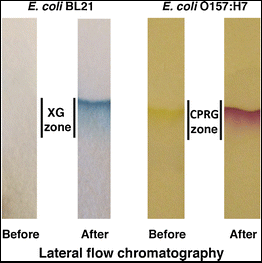
\includegraphics{./img/ecoli.png}\\



Avant de pouvoir trouver les épitopes communs de toutes les souches de E. coli, il va falloir faire un alignement de séquence avec toutes les souches afin de faire ressortir les régions de séquences similaires.

Un alignement de séquence est une manière de représenter deux ou plusieurs séquences de macromolécules biologiques les unes sous les autres, de manière à en faire ressortir les régions homologues ou similaires. L'objectif d'un alignement de séquence est donc d'identifier les zones de concordance.

 L'alignement devra être un alignement multiples car nous avons bien plus que deux souches à analyser. Il existe déjà plusieurs algorithmes d'alignement de séquence multiple, nous allons comparer les différents logiciels qui proposent un MSA(Multiple Sequence Alignements) ci-dessous.
 
 
\begin{itemize}
  \item ClustalW2 : Un des premiers logiciels de MSA datant de 1988. Les auteurs cite que le logiciel est clairement dépassé. Nous n'allons donc pas utilisé ce logiciel. 
  \item MAFFT version 7 : possède un des algorithmes les plus rapides à ce jour et est donc l'un des plus utilisés. Les alignements générés par cet outil sont de bonne qualité mais possède certaines fois quelques petites erreurs.
  
  \item MUSCLE: est un peu plus lent que MAFFT mais rien de très grave. Son alignement est un poile meilleur que celui de MAFFT. En plus de cela nous l'avons utilisé pendant notre laboratoire 2. Nous sommes déjà habitués à ce logiciel. 

	\item Clustal Omega: il utilise une méthode d'alignement progressive tandis que Muscle utilise une méthode d'alignement itérative. L'avantage de la méthode itérative est que l'on peut revenir au calcule précédent du meilleur alignement. Il y'a donc plus d'erreur possible avec une méthode d'alignement progressive que itérative.
	
\end{itemize}

Nous allons donc nous orienter vers l'algorithme MUSCLE pour pouvoir aligner nos séquences de façon efficace. MAFFT aurait aussi pu être un choix mais le fait que nous sommes déjà familiarisé avec MUSCLE fait pencher la balance. 

  \section{Réalisation}
  
    \subsection{Analyse de OmpF porin}
    
    \subsection{Critères de sélection d'épitope}
  
  \section{Conclusion}

  
\bibliography{biblio}
\nocite{*}

\end{document}

